\section{ОБЗОР ЛИТЕРАТУРЫ}
\label{sec:domain}

\subsection{Обзор существующих аналогов}

На этапе исследования и проектирования модуля были тщательно изучены существующие аналоги. Так как в последние годы наблюдается растущий интерес к генерации и редактированию изображения на основе текстовых описаний, то приложений-аналогов было найдено достаточно большое количество, однако большинство из них ориентированы на генерация изображения без возможности выделения области на изображении. Одинм из примеров приложения которое позволяет 

\subsubsection{Adobe Firefly}

Adobe Firefly~\cite{firefly} (рисунок~\ref{domain::adobe}) представляет собой инструмент генеративного искусственного интеллекта от компании Adobe, созданный специально для творческих нужд, кейсов и рабочих процессов. Этот инструмент обучался на изображениях Adobe Stock, контенте с открытой лицензией и контенте из общественного достояния, благодаря чему его можно безопасно использовать в коммерческих целях. Firefly доступен как самостоятельное веб-приложение, предлагая новые способы идеализации, создания и общения, значительно улучшая творческие рабочие процессы.

\begin{figure}[ht]
    \centering
    
\includegraphics[width=1.0\linewidth]{Adobe-Firefly.jpg}
    \caption{Adobe Firefly}
    \label{domain::adobe}
\end{figure}

Использование искусственного интеллекта в Adobe Firefly охватывает три ключевых направления: создание визуальных изображений, генерацию текстовых эффектов, и модификацию цвета векторных график.

Чтобы сгенерировать изображение в Adobe Firefly, пользователь должен предоставить текстовое описание. Чем оно более детализировано, тем более точным окажется результат. В настоящее время запросы принимаются исключительно на английском языке. После создания изображения, искусственный интеллект предоставляет возможности для его дальнейшей настройки: от редактирования в графическом редакторе до изменения формата с квадратного на широкоформатный. Пользователь может разбить изображение на отдельные слои и редактировать их по отдельности, применять различные фильтры, корректировать уже готовые изображения и многое другое. В конце работы изображения доступны для скачивания.

Преимущества которые можно выделить у данной модели:
\begin{itemize}
    \item создание уникальных изображений по запросу;
    \item изменение полученных изображений в редакторе;
    \item обработка результата дополнительными запросами;
    \item изменение отдельных элементов изображений;
    \item понимает перспективу, её линии, свет, что делает изображение более естественным;
    \item создание изображения из наброска.
\end{itemize}

Недостатки Adobe Firefly:
\begin{itemize}
    \item доступен только по подписке;
    \item отправляет изображение на сервер что может вызвать утечки;
    \item наличие цензуры;
    \item генерирует изображение 1024х1024 и потом масштабирует его, из-за чего изображение больших размеров может получиться замыленым. 
\end{itemize}

\subsubsection{DALL·E}

DALL·E~\cite{dalle} (рисунок~\ref{domain::dalle})~-- продукт разработанный компанией OpenAI, представляет собой революционный инструмент генеративного искусственного интеллекта, способный создавать изображения и иллюстрации из текстовых описаний.

\begin{figure}[ht]
    \centering
    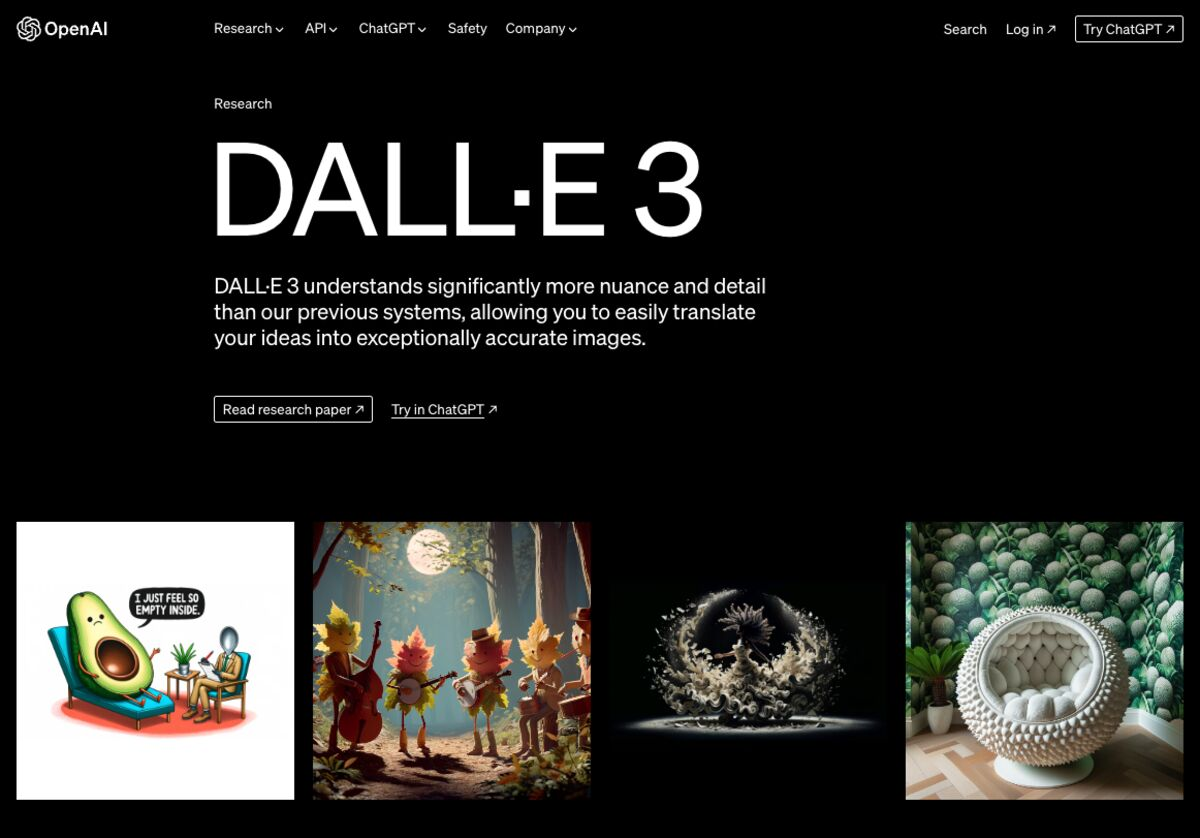
\includegraphics[width=.7\linewidth]{DALL-E.png}
    \caption{DALL·E}
    \label{domain::dalle}
\end{figure}

Этот инструмент может не только создавать уникальные изображения и иллюстрации из текстовых подсказок, но и модифицировать существующие изображения, добавляя элементы, изменяя контекст или адаптируя стиль под указанные требования. Такая функциональность открывает новые горизонты для дизайнеров, художников, маркетологов и всех творческих личностей, предоставляя им мощный инструмент для воплощения их самых смелых идей.

Интеграция DALL·E с ChatGPT также заслуживает особого внимания. Это сочетание позволяет пользователям формулировать свои запросы естественным языком, делая процесс создания изображений еще более интуитивным и доступным. ChatGPT, обладая способностью к пониманию и обработке сложных текстовых запросов, может трансформировать описания пользователей в детализированные инструкции для DALL·E, что в итоге приводит к созданию более точных и соответствующих ожиданиям изображений.

Основными преимуществами можно выделить:
\begin{itemize}
    \item тонко схватывает все нюансы запросов;
    \item активно развивается;
    \item этические и авторские проблемы.
\end{itemize}

Недостатки:
\begin{itemize}
    \item отсутствует возможность менять масштаб;
    \item доступно только по платной подписке;
    \item ограниченность датасета.
\end{itemize}

\subsection{Обзор средств разработки}

\subsubsection{Обзор языка программирования}

В качестве языка разработки был выбран интерпретируемый язык программирования Python~\cite{python}.

Python~-- это мощный, переносимый, простой в использовании и свободно распространяемый язык. Программисты, работающие в самых  разных областях, считают, что ориентация Python на эффективность разработки и высокое качество программного обеспечения дает ему стратегическое преимущество как в маленьких, так и в крупных проектах.

В составе Python поставляется большое число собранных и переносимых функциональных возможностей, известных как 
стандартная библиотека. Эта библиотека предоставляет массу возможностей, востребованных в прикладных программах, начиная от поиска текста по шаблону и заканчивая сетевыми функциями. Кроме того, Python допускает расширение как за счет ваших собственных библиотек, так и за счет библиотек, созданных сторонними разработчиками. Из числа сторонних разработок можно назвать инструменты создания веб-сайтов, программирование математических вычислений, доступ к последовательному порту, разработку игровых программ и многое другое. Например, расширение NumPy позиционируется как свободный и более мощный эквивалент системы программирования математических вычислений Mathlab.

\subsubsection{Обзор среды разработки}

В качестве среды разработки был выбран продукт компании Google~-- Google Colab~\cite{colab}, или Colaboratory (рисунок~\ref{domain::colab}). 

\begin{figure}[ht]
    \centering
    
\includegraphics[width=1\linewidth]{Google-Colaboratory.png}
    \caption{Google Colab}
    \label{domain::colab}
\end{figure}

Google Colab представляет собой бесплатную среду разработки, которая позволяет пользователям писать и выполнять код Python прямо в браузере. Этот инструмент особенно полезен для студентов, исследователей и разработчиков в области машинного обучения и анализа данных, поскольку он обеспечивает легкий доступ к мощным вычислительным ресурсам, таким как GPU и TPU, без необходимости сложной настройки.

Google Colab поддерживает множество популярных библиотек и фреймворков для машинного обучения, таких как TensorFlow, PyTorch, Keras, обеспечивая легкость импорта и использования в проектах. 

Одной из ключевых особенностей Colab является его способность к совместной работе в реальном времени, аналогичной Google Docs, что позволяет нескольким пользователям одновременно работать над одним и тем же документом, упрощая тем самым обмен знаниями и совместную работу. Кроме того, благодаря тесной интеграции с Google Drive, доступ к данным, их хранение и распространение становятся значительно удобнее.

\subsection{Нейронные сети}

В качестве основной технологии для обеспечения заданной функциональности выбраны искусственные нейронные сети. Данное решение обусловлено способностями сети к параллельной и распределенной обработки информации.

Нейронные сети представляют собой сложные математические модели, вдохновленные структурой и функционированием человеческого мозга, и являются одним из основных инструментов в области искусственного интеллекта и машинного обучения. Они состоят из множества узлов, называемых нейронами, которые связаны друг с другом и организованы в слои: входной слой, который принимает исходные данные, один или несколько скрытых слоев, где происходит обработка данных, и выходной слой, который представляет результат обработки.

Структура простейшей нейронной сети представлена на рисунке~\ref{domain::simple-nn}. Зеленым цветом обозначены нейроны входного слоя, голубым~-- нейроны скрытого слоя, желтым~-- нейрон(ы) выходного слоя.

\begin{figure}[ht]
    \centering
    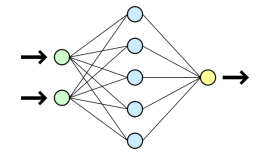
\includegraphics[width=0.55\linewidth]{Simple-NN.png}
    \caption{Структура простейшей нейронной сети}
    \label{domain::simple-nn}
\end{figure}

Каждый нейрон в этих слоях получает входные данные, которые взвешиваются~-- этот процесс определяет важность входящих сигналов. Веса этих входных данных затем суммируются, и к сумме может быть добавлено смещение, которое помогает регулировать порог, при котором нейрон будет активирован. Эта взвешенная сумма затем проходит через функцию активации, которая определяет, будет ли и в какой степени нейрон передавать сигнал дальше. Функции активации добавляют нелинейность в обработку данных, что критически важно для возможности нейронной сети учиться и адаптироваться к сложным задачам, таким как распознавание образов или обработка естественного языка~\cite{speach_neural}.

Обучение нейронных сетей обычно происходит через процесс, известный как обратное распространение ошибки, при котором модель сначала делает предположение о выходных данных, затем сравнивает свое предположение с фактическими результатами и использует разницу между этими значениями, чтобы сделать корректировки в весах и смещениях своих нейронов. Этот процесс повторяется многократно, и с каждым повторением модель становится всё более точной в своих предсказаниях.

Глубокое обучение~-- это подкатегория машинного обучения, которая использует нейронные сети с множеством скрытых слоев, что позволяет обрабатывать данные на значительно более глубоком уровне. Это дает возможность моделям выявлять и интерпретировать сложные и абстрактные паттерны в данных. Например, в процессе анализа изображения выход первого слоя нейронной сети может быть расценен как базовые абстракции вида – различные линии и углы. Следующие этапы усложняют эту картину: линии объединяются в формы, а формы группируются в более крупные комплексы. В итоге, на основе собранной информации, глубокая нейронная сеть способна определить, что эти комплексные категории образуют определенный объект или сцену. Так, более сложная структура категорий дает возможность глубоким нейронным сетям эффективно решать задачи от автоматического распознавания речи и изображений до создания самообучающихся систем, способных моделировать человеческий язык и даже создавать искусство.

Нейронные сети нашли широкое применение в самых разных областях современной жизни. Примеры их использования варьируются от автоматического распознавания образов и обработки естественного языка до более специализированных применений, таких как предсказание финансовых рынков и управление автономными транспортными средствами.

В области здравоохранения, например, нейронные сети используются для анализа медицинских изображений~\cite{mrt_neural}, таких как МРТ и рентгеновские снимки, чтобы помочь в диагностике заболеваний на ранних стадиях. В финансах они помогают анализировать большие объемы данных для предсказания тенденций рынка и поведения акций~\cite{busines_neural}, что делает их неоценимым инструментом для трейдеров и инвесторов. В автомобильной индустрии нейронные сети лежат в основе систем автономного вождения~\cite{car_neural}, обучаясь распознавать и интерпретировать окружающую дорожную обстановку, что обеспечивает безопасность и эффективность передвижения.

История развития нейронных сетей уходит корнями в изучение нейронов человеческого и животного мозга. Задумка о создании компьютерных моделей, способных воспроизводить функции мозга, существует уже давно и стала ключевым двигателем исследований в данной области. В настоящее время нейронные сети находят широкое применение в различных сферах, включая компьютерное зрение, где они идентифицируют объекты на изображениях с поразительной точностью, даже превосходя в некоторых аспектах человеческие способности. В области обработки естественного языка эти технологии позволяют моделям понимать, создавать тексты и отвечать на вопросы, используя естественный язык.

Тем не менее, нейронные сети не способны полностью заместить человеческий интеллект, особенно когда речь идет о принятии решений в ситуациях, требующих учета моральных и этических норм. В то время как они могут анализировать обширные массивы данных и выявлять в них закономерности, недоступные для человеческого восприятия, нейронные сети могут быть не идеальным инструментом для некоторых задач. Однако их способность к анализу и принятию решений на основе обнаруженных закономерностей демонстрирует огромный потенциал этих технологий, которые уже сегодня активно внедряются во многие аспекты человеческой деятельности, обещая дальнейшие инновации и улучшения в будущем.

\subsection{Основные архитектуры нейронных сетей}

Многообразие архитектур нейронных сетей специально разработано для выполнения различных задач в области машинного обучения. Тем не менее, среди них можно выделить несколько ключевых архитектур, наиболее часто применяемых на практике.

\subsubsection{Сверточные нейронные сети}

Сверточная нейронная сеть~-- специальная архитектура искусственных нейронных сетей, предложенная Яном Лекуном в 1988 году и нацеленная на эффективное распознавание образов, входит в состав технологий глубокого обучения. Архитектура сети представлена на рисунке~\ref{domain::convolutional-nn}

\begin{figure}[ht]
    \centering
    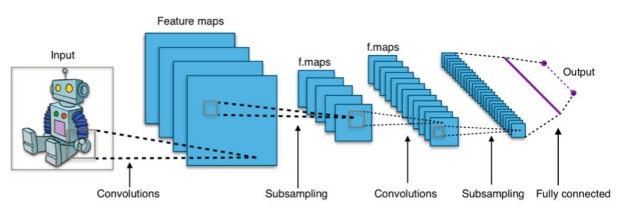
\includegraphics[width=.88\linewidth]{Convolutional-NN.png}
    \caption{Архитектура сверточной нейронной сети}
    \label{domain::convolutional-nn}
\end{figure}

Сверточный слой нейронной сети представляет из себя операцию свертки, которая применяется к выходам с предыдущего слоя, где веса ядра свертки являются обучаемыми параметрами. Слой подвыборки (pooling) принимает на входы результаты свертки с предыдущего слоя и сжимает их. Делается это с целью выделения низкоуровневых признаков и понижения размера данных. В качестве функции сжатия может выступать:

\begin{itemize}
    \item среднее арифметическое элементов по окну;
    \item максимальное значение по окну.
\end{itemize}

Чаще всего применяется максимальное значение по окну. 

Для обучения сверточной нейронной сети используется один из подвидов алгоритма обратного распространения ошибки (backpropagation), что позволяет им настраивать параметры фильтров и полносвязных слоев (fully connected layers) для оптимальной классификации или регрессии. Данный алгоритм относится к методам обучения с учителем.

Таким образом, сверточная нейронная сеть извлекает локальные признаки из изображения, например ребра, углы, текстуры и т.д.

Одной из причин, почему сверточные нейронные сети являются такими эффективными, является их способность обнаруживать иерархические признаки изображения на разных уровнях абстракции. Например, на первом уровне сеть может выделять ребра и текстуры, на следующем~-- формы и контуры объектов, а на последующих уровнях~-- более сложные и абстрактные признаки, такие как фигуры и части объектов.

\subsubsection{Сети прямого распространения}

Сети прямого распространения (feedforward neural networks)~-- являются одной из базовых и широко используемых архитектур нейронных сетей. Эти сети структурированы в виде последовательных слоёв, где каждый нейрон слоя связан с каждым нейроном следующего слоя, но нет обратных связей. В общем случае каждый нейрон в скрытом слое 
может получать входные данные от всех нейронов предыдущего слоя, а каждый нейрон в выходном слое получает входные данные от всех нейронов последнего скрытого слоя.

На рисунке~\ref{domain::feedforward-nn} представлена структура сетей прямого распространения, включающая три основных типа слоёв: входной слой, один или несколько скрытых слоёв и выходной слой. Входной слой принимает исходные данные, скрытые слои обрабатывают данные, применяя различные веса и функции активации, а выходной слой производит итоговый результат или предсказание.

\begin{figure}[ht]
    \centering
    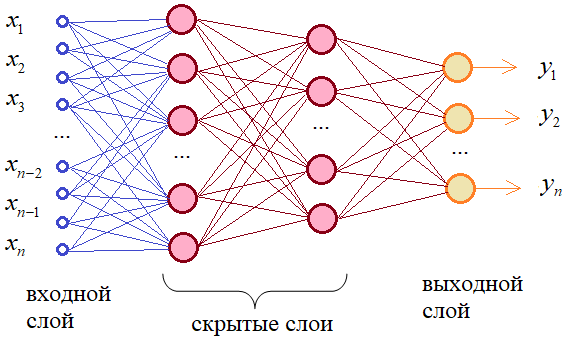
\includegraphics[width=0.6\linewidth]{Feedforward-NN.png}
    \caption{Архитектура сети прямого распространения}
    \label{domain::feedforward-nn}
\end{figure}

Сети прямого распространения находят применение в широком спектре задач машинного обучения, включая классификацию, регрессию, и прогнозирование. Они являются основой для многих более сложных архитектур и техник машинного обучения, подчёркивая их важность в исследованиях и практическом применении. Сети прямого распространения могут точно классифицировать изображения, тексты и другие типы данных, а также предсказывать числовые значения, как в оценке стоимости недвижимости. Также они анализируют исторические данные для прогнозирования будущих событий, обнаруживая тонкие взаимосвязи в данных.

Их универсальность и мощь делают сети прямого распространения не просто инструментом для решения задач, но и фундаментом для исследований и разработок в области искусственного интеллекта, подчёркивая их значимость и потенциал в сфере машинного обучения.

\subsubsection{Рекуррентные нейронные сети}

Рекуррентные нейронные сети (RNN)~-- это класс нейронных сетей, специально разработанный для работы с последовательными данными, такими как временные ряды, тексты и аудио. 

Основным элементом RNN является рекуррентный блок представленные на рисунке~\ref{domain::recurrent-nn}, который повторяется на каждом временном шаге и принимает на вход текущий элемент последовательности и скрытое состояние с предыдущего шага. Рекуррентный блок вычисляет новое скрытое состояние, которое затем передается на следующий шаг. Таким образом, RNN сохраняют информацию о предыдущих элементах последовательности и могут использовать ее для принятия решений на текущем шаге.

\begin{figure}[ht]
    \centering
    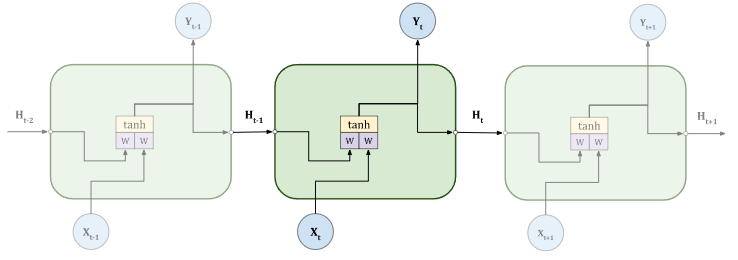
\includegraphics[width=0.9\linewidth]{Recurrent-NN.png}
    \caption{Рекуррентный блок}
    \label{domain::recurrent-nn}
\end{figure}

В обработке естественного языка RNN могут учитывать последовательность слов для более точного определения их значений или для генерации текста. В области прогнозирования временных рядов, таких как финансовые данные или погодные условия, RNN используются для анализа предыдущих значений и предсказания будущих тенденций. Однако RNN сталкиваются с проблемой затухания или взрыва градиентов при обработке длинных последовательностей, что ограничивает их способность улавливать долгосрочные зависимости. Для решения этих проблем были разработаны более продвинутые вариации RNN, такие как LSTM (Long Short-Term Memory) и GRU (Gated Recurrent Unit), которые включают механизмы забывания и обновления информации, позволяя эффективно работать с долгосрочными зависимостями в данных. Эти улучшения расширяют возможности RNN, делая их мощным инструментом для широкого спектра приложений в машинном обучении и искусственном интеллекте.

\subsubsection{Генеративно-состязательные сети}

Генеративно-состязательные сети или Generative Adversarial Networks (GANs), это класс алгоритмов машинного обучения. Эти алгоритмы состоят из двух сетей: генеративной сети и дискриминативной сети, которые обучаются одновременно в процессе игры с нулевой суммой, отсюда и название <<состязательные>>. Архитектура сети представлена на рисунке~\ref{domain::gan-nn}

\begin{figure}[ht]
    \centering
    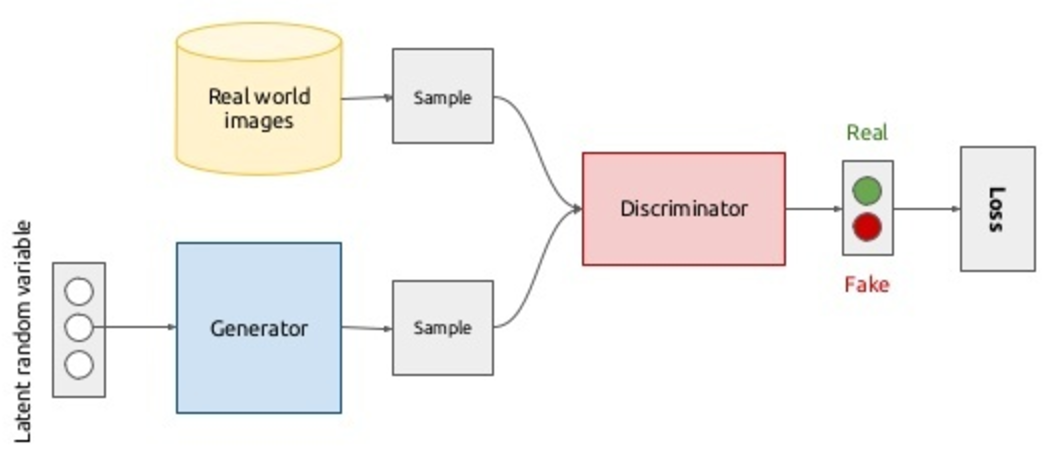
\includegraphics[width=0.93\linewidth]{gan-nn.png}
    \caption{Архитектура генеративно-состязательной сети}
    \label{domain::gan-nn}
\end{figure}

Генеративная сеть стремится генерировать данные, максимально похожие на реальные. Она пытается <<обмануть>> дискриминативную сеть, создавая все более убедительные подделки. В качестве входных данных она использует случайный шум, и через множество итераций обучения учится преобразовывать этот шум в данные, которые трудно отличить от настоящих.

Дискриминативная сеть анализирует как подлинные данные, так и данные, сгенерированные генеративной сетью, и старается отличить настоящие данные от подделок. Ее задача~-- правильно классифицировать входные данные как <<реальные>> или <<сгенерированные>>.

В процессе обучения генеративная сеть пытается улучшить свою способность генерировать подделки, становясь всё более изощренной в имитации реальных данных, в то время как дискриминативная сеть старается стать лучше в распознавании подделок. Этот процесс можно сравнить с игрой в кошки-мышки, где с каждым раундом обе сети улучшают свои способности.

Генеративно-состязательные сети нашли широкое применение во многих областях, включая:

\begin{itemize}
    \item создание фотореалистичных изображений лиц людей, которые на самом деле не существуют;
    \item генерация арт-контента, музыки и текстов;
    \item улучшение качества изображений;
    \item перенос стилей с одного изображения на другое.
\end{itemize}

Генеративно-состязательные сети продолжают развиваться и находить новые применения благодаря своей уникальной способности генерировать данные, очень похожие на реальные, что открывает новые горизонты для искусственного интеллекта и машинного обучения.

\subsubsection{Автокодировщики}

Автокодировщики представляют собой тип архитектуры нейронных сетей, задействованный для обнаружения не очевидных закономерностей в данных и их сжатия. Эта структура включает в себя энкодер, который трансформирует данные во внутреннее, или скрытое, представление, и декодер, который затем реконструирует данные, исходя из этого скрытого состояния.

\begin{figure}[ht]
    \centering
    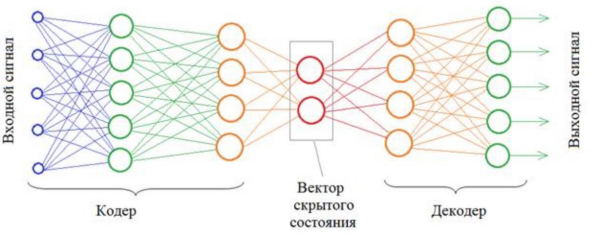
\includegraphics[width=0.8\linewidth]{Autoencoders.png}
    \caption{Архитектура автокодировщика}
    \label{domain::autoencoders}
\end{figure}

Основная концепция автокодировщиков, архитекрута, которого представлена на рисунке~\ref{domain::autoencoders}, состоит в том, что они стремятся точно воспроизвести на выходе те же данные, что и поданы на вход. Это достигается за счет того, что автокодировщик «обучается» выделять ключевые характеристики входящих данных, которые затем используются для их кодирования и последующего декодирования. В процессе работы данные сначала передаются через энкодер, затем через декодер, при этом на выходе должны получаться данные, максимально приближенные к оригиналу. Разница между оригинальными и восстановленными данными анализируется, и на основе этой ошибки происходит корректировка весов.

Автокодировщики находят применение в широком спектре задач. Эти модели могут быть использованы для компрессии данных, очистки от шумов, реконструкции изображений и создания новых данных.

\subsection{История и развитие генеративно-состязательных сетей}

Генеративная Состязательная Сеть (GAN)~-- одна из самых интересных идей в машинном обучении за последние десять лет. На высоком уровне GAN~-- это нейронные сети, которые учатся генерировать реалистичные образцы данных, на которых они обучались. Например, имея фотографии рукописных цифр, GAN узнают, как создавать реалистичные фотографии большего количества рукописных цифр. Что еще более впечатляюще, GAN могут даже научиться создавать реалистичные фотографии людей, такие как приведенные на рисунке~\ref{domain::gan_faces}. несмотря на то, что эти лица не принадлежат ни одному реальному человеку.

\begin{figure}[ht]
    \centering
    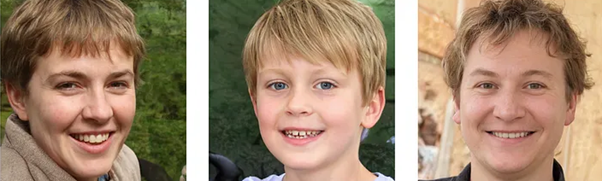
\includegraphics[width=1\linewidth]{gan_faces.png}
    \caption{Человеческие лица, сгенерированные GAN. Ни одно из вышеперечисленных лиц не является реальным}
    \label{domain::gan_faces}
\end{figure}

Для обучения GAN нужен только набор данных (изображений, аудио и т. п.), которые хочется скопировать или имитировать. Сеть сама определит способы создания новых данных, которые будут выглядеть как данные из полученного сетью набора данных.
Архитектура GAN включает две состязающиеся между собой нейросети. Отсюда и слово «состязательные» в названии. Эти две сети называются генеративной (G) и дискриминационной (D) или просто генератором и дискриминатором соответственно. Задача генератора – изучить функцию генерации данных, начиная со случайного шума. Дискриминатор должен определить, является ли образец данных «подлинным». При этом «подлинностью» считается принадлежность к образцам исходного набора данных. Это позволяет измерить эффективность модели и отрегулировать её параметры. Обе нейросети обучаются одновременно.
В GAN генератор~-- это нейронная сеть, которая изучает базовое распределение данных. Чтобы быть более конкретным, как показано на рисунке 3.20,  генератор принимает в качестве входных данных случайное распределение (также известное как «шум» в литературе по GAN) и изучает функцию отображения, которая отображает входные данные в желаемый результат, который является фактическим базовым распределением данных.

\subsection{Преимущества и ограничения нейронных сетей}

Нейронные сети представляют собой мощный инструмент в современном мире искусственного интеллекта, благодаря своей способности анализировать, интерпретировать и прогнозировать результаты на основе больших и сложных наборов данных. Они нашли широкое применение в различных областях, от распознавания речи до компьютерного зрения и автоматического перевода. Давайте подробнее рассмотрим основные преимущества нейронных сетей:

\begin{enumerate_num}
    \item Обработка сложных данных. Нейронные сети могут обрабатывать большой объем данных, включая неструктурированные данные, такие как изображения, аудио и текст. Они также могут обрабатывать данные в реальном времени, что делает их полезными в таких областях, как машинное зрение, обработка речи и автоматический перевод.
    \item Адаптивность. Нейронные сети могут быть обучены для решения широкого спектра задач. Они могут адаптироваться к новым условиям и изменяющейся среде. Это позволяет им достигать высокой точности в решении различных задач.
    \item Распараллеливание. Нейронные сети могут быть распараллелены на несколько процессоров, что позволяет им обрабатывать большие объемы данных и решать сложные задачи, такие как распознавание речи и обработка изображений.
    \item Автоматизация. Нейронные сети могут автоматизировать многие задачи, которые ранее требовали человеческого участия. Например, они могут автоматически распознавать образцы в данных, обнаруживать аномалии или предсказывать будущие значения.
    \item Обучение на больших данных. Нейронные сети могут быть обучены на больших наборах данных, что позволяет им улучшать свою точность и качество решения задач. Большие наборы данных также позволяют нейронным сетям выявлять скрытые закономерности в данных.
    \item Гибкость. Нейронные сети могут быть настроены для решения широкого спектра задач, включая классификацию, регрессию, кластеризацию и многие другие. Они также могут быть изменены и оптимизированы для различных задач.
\end{enumerate_num}

В целом, нейронные сети обладают множеством преимуществ, которые делают их полезными в широком спектре областей. Однако они также имеют некоторые ограничения, о которых стоит упомянуть:

\begin{enumerate_num}
    \item Необходимость больших объемов данных. для обучения нейронной сети требуется большое количество данных. Если данных недостаточно, сеть может недообучиться, что приведет к плохой производительности.
    \item Вычислительная сложность. Некоторые типы нейронных сетей требуют больших вычислительных ресурсов, таких как GPU, чтобы достичь хороших результатов. Это может быть проблематично для компаний или исследовательских групп с ограниченными вычислительными ресурсами.
    \item Необходимость экспертных знаний. Для разработки эффективной нейронной сети требуются экспертные знания в области математики, статистики и программирования. Это может быть вызовом для тех, кто только начинает работать в этой области.
    \item Трудности интерпретации результатов. Нейронные сети могут давать высокую точность в предсказаниях, но иногда сложно объяснить, как они пришли к этим результатам. Это может быть проблематично, если требуется обосновать принятые решения на основе работы нейронной сети.
    \item Неустойчивость к изменениям в данных. Нейронные сети могут быть чувствительны к изменениям в данных. Например, если данные содержат выбросы или ошибки, это может привести к неправильным предсказаниям.
\end{enumerate_num}

Необходимо учитывать эти недостатки при выборе подходящей нейронной сети и внедрении ее в практические приложения.

\subsection{Использование нейронных сетей в различных областях}

Нейронные сети~-- это мощный инструмент в области машинного обучения, который используется во многих областях для решения различных задач. Они позволяют анализировать данные, выделять в них закономерности и предсказывать результаты. Благодаря своей гибкости и универсальности, нейронные сети нашли свое применение в самых разных областях~-- от медицины и финансов до игровой индустрии и анализа социальных сетей. Рассмотрим некоторые из них:
Обработка естественного языка (Natural Language Processing, NLP). Нейронные сети широко используются в обработке естественного языка для решения различных задач, таких как машинный перевод, сентимент-анализ, определение языка и генерация текста. Например, нейронная сеть GPT-4 (Generative Pre-trained Transformer 4) используется для генерации текста с высоким качеством, в том числе для создания статей, новостей и рецензий.

Медицина. Нейронные сети также нашли свое применение в медицине. Они используются для анализа медицинских изображений, таких как рентгеновские снимки и снимки магнитно-резонансной томографии (МРТ), для диагностики заболеваний и предсказания результатов лечения. Например, нейронная сеть CAD (Computer-Aided Detection) используется для автоматической диагностики рака молочной железы на основе медицинских изображений.

Финансы. Нейронные сети также применяются в финансовой отрасли для анализа данных, прогнозирования цен на акции и валюты, и для выявления мошенничества. Например, нейронная сеть LSTM (Long Short-Term Memory) используется для прогнозирования цен на акции и другие финансовые индикаторы.

Рекомендательные системы. Нейронные сети также используются в рекомендательных системах, которые помогают пользователям выбирать товары и услуги на основе их предпочтений и истории. Например, нейронная сеть Netflix используется для рекомендации фильмов и телешоу на основе просмотров и оценок.

Робототехника. Нейронные сети также используются в робототехнике для управления и обучения роботов. Например, нейронные сети могут использоваться для обучения роботов-манипуляторов, чтобы они могли выполнять различные задачи, такие как сборка и упаковка товаров.

Автоматическое управление производственными процессами. Нейронные сети также применяются для автоматического управления производственными процессами, чтобы повысить эффективность и качество производства. Например, нейронные сети могут использоваться для прогнозирования времени остановки оборудования и для управления подачей материалов на производственной линии.

Игровая индустрия. Нейронные сети также нашли свое применение в игровой индустрии для улучшения графики, искусственного интеллекта и игрового процесса. Например, нейронные сети могут использоваться для генерации реалистичных графических изображений и для создания более умных врагов в компьютерных играх.

Анализ социальных сетей. Нейронные сети также используются для анализа социальных сетей для выявления тенденций, прогнозирования поведения пользователей и идентификации ключевых лидеров. Например, нейронная сеть PageRank используется для ранжирования страниц в поисковых системах на основе их важности и релевантности.

Это лишь некоторые из областей, где нейронные сети нашли свое применение. На сегодняшний день они являются одним из самых мощных инструментов в машинном обучении и имеют огромный потенциал для решения самых разнообразных задач.


\subsection{Постановка задачи}

Цель данного дипломного проекта заключается в разработке программного модуля, который предоставляет возможность редактировать изображения на основе текстовых описаний. Для этого предлагается объединить две нейронные сети: первая, которая с помощью сегментации выделяет объекты на изображении, а вторая~-- диффузионная модель, которая генерирует новое изображение, отредактировав выбранный пользователем объект на другой с учетом текстового описания. 

Данный подход имеет большой потенциал в таких областях, как графический дизайн, архитектура, видеопроизводство и даже в маркетинг. В дизайне он может использоваться для быстрого создания и наложения новых деталей на изображение. В архитектуре позволяет оптимизировать дизайн, ускоряя разработку и способствуя инновациям. В видеопроизводстве позволяет добавлять сложные визуальные эффекты, экспериментировать с окружением и тем самым повышать его привлекательность. В маркетинге и рекламе алгоритм обеспечивает более точную персонализацию и целенаправленность кампаний, укрепляя связь с аудиторией.

В результате изучения специфики темы, анализа разнообразия типов и архитектур нейронных сетей, а также исследования их применений в различных областях, было установлено что для реализации дипломного проекта необходимо реализовать следующие задачи:

\begin{enumerate_num}
    \item Выбор метода сегментации изображений.
    \item Выбор метода для генерации изображений.
    \item Разработка архитектуры для взаимодействия двух нейронных сетей для достижения поставленной задачи. 
    \item Реализация программного модуля и тестирование его на разных примерах.
    \item Написание удобного интерфейса для использования данного модуля и возможности интеграции его в различные приложения.
    \item Оценка возможности применения данного модуля в разных сферах жизни.
\end{enumerate_num}
